%%%%%%%%%%%%%%%%%%%%%%%%%%%%%%%%%%%%%%%%%%%%%%%%%%%%%%%%%%%%%%%%%%%%%%%%%%%%%%%%
%2345678901234567890123456789012345678901234567890123456789012345678901234567890
%        1         2         3         4         5         6         7         8

\documentclass[letterpaper, 10 pt, conference]{ieeeconf}  % Comment this line out if you need a4paper

%\documentclass[a4paper, 10pt, conference]{ieeeconf}      % Use this line for a4 paper

\IEEEoverridecommandlockouts                              % This command is only needed if 
                                                          % you want to use the \thanks command

\overrideIEEEmargins                                      % Needed to meet printer requirements.

%In case you encounter the following error:
%Error 1010 The PDF file may be corrupt (unable to open PDF file) OR
%Error 1000 An error occurred while parsing a contents stream. Unable to analyze the PDF file.
%This is a known problem with pdfLaTeX conversion filter. The file cannot be opened with acrobat reader
%Please use one of the alternatives below to circumvent this error by uncommenting one or the other
%\pdfobjcompresslevel=0
%\pdfminorversion=4

% See the \addtolength command later in the file to balance the column lengths
% on the last page of the document

% The following packages can be found on http:\\www.ctan.org
\usepackage{graphics} % for pdf, bitmapped graphics files
\usepackage{graphicx}
\usepackage{subcaption}
\usepackage{amsmath}
\usepackage{makecell} 
%\usepackage{epsfig} % for postscript graphics files
%\usepackage{mathptmx} % assumes new font selection scheme installed
%\usepackage{times} % assumes new font selection scheme installed
%\usepackage{amsmath} % assumes amsmath package installed
%\usepackage{amssymb}  % assumes amsmath package installed

\title{\LARGE \bf
AI-based HRI Group 1 Project Report: \\HRI with Dancing Robot Arm}

%  

\author{Gwanwoo Choi$^{1*}$, Haechan Chong$^{2*}$, Hyeonbin Lee$^{3*}$, Jeonghwan Song$^{2*}$, Jiwon Kim$^{4*}$, Minseong Boo$^{2*}$ %<-this % stops a space
\thanks{*Alphabet order.}% <-this % stops a space
\thanks{$^{1}$Department of Computer Science and Engineering, UNIST, Ulsan, South
Korea.{\tt\small \{cgw1999\}@unist.ac.kr}}
\thanks{$^{2}$Graduate School of Artificial Intelligence, UNIST, Ulsan, South Korea.{\tt\small \{atlantic0924, jeonghwansong, b.ms\}@unist.ac.kr}}
\thanks{$^{3}$Department of Mechanical Engineering, UNIST, Ulsan, South
Korea. {\tt\small \{bin2915\}@unist.ac.kr}}
\thanks{$^{4}$Department of Electrical Engineering, UNIST, Ulsan, South
Korea. {\tt\small \{jiwonkim01\}@unist.ac.kr}}
}


\begin{document}

\maketitle
\thispagestyle{empty}
\pagestyle{empty}


%%%%%%%%%%%%%%%%%%%%%%%%%%%%%%%%%%%%%%%%%%%%%%%%%%%%%%%%%%%%%%%%%%%%%%%%%%%%%%%%
\begin{abstract}

In this project, we design a framework for human-robot interaction (HRI) with a dancing robot arm. There is a lot of research about robot dance, even if it is not a humanoid robot, and human-robot interaction using large language model (LLM). So, we determine our project topic combining human-root interaction using LLM and robot dancing to non-humanoid robot, Koch v1.1. To do so, we implement functions such as robot conversation with human, recognizing feeling of human for music recommendation, human movement detection, robot dance for human, and robot dance with human. To evaluate our framework, we measure beat alignment between music and both human, robot dance motion, and conduct user survey. Experiment results show that our framework makes alignment between robot dance and music well and the robot's dance fits the music but does not closely mimic human movements.

\end{abstract}


%%%%%%%%%%%%%%%%%%%%%%%%%%%%%%%%%%%%%%%%%%%%%%%%%%%%%%%%%%%%%%%%%%%%%%%%%%%%%%%%
\section{INTRODUCTION}

tmp

\section{METHODOLOGY}

In this section, we present how to generate robot dance with human-robot interaction. Fig. \ref{fig:overview} shows the overview of our framework. In our framework, the robot selects the music by interacting with the human. Once the music is selected, human dance motion is generated by EDGE \cite{tseng2023edge} model, which is one of the state-of-the-art model for human dance generation that creates realistic, physically-plausible dance motions based on input music. Finally, the robot dance motion is generated by matching the parts of human's body to the joint of robot.

\begin{figure}[h]
    \centering
    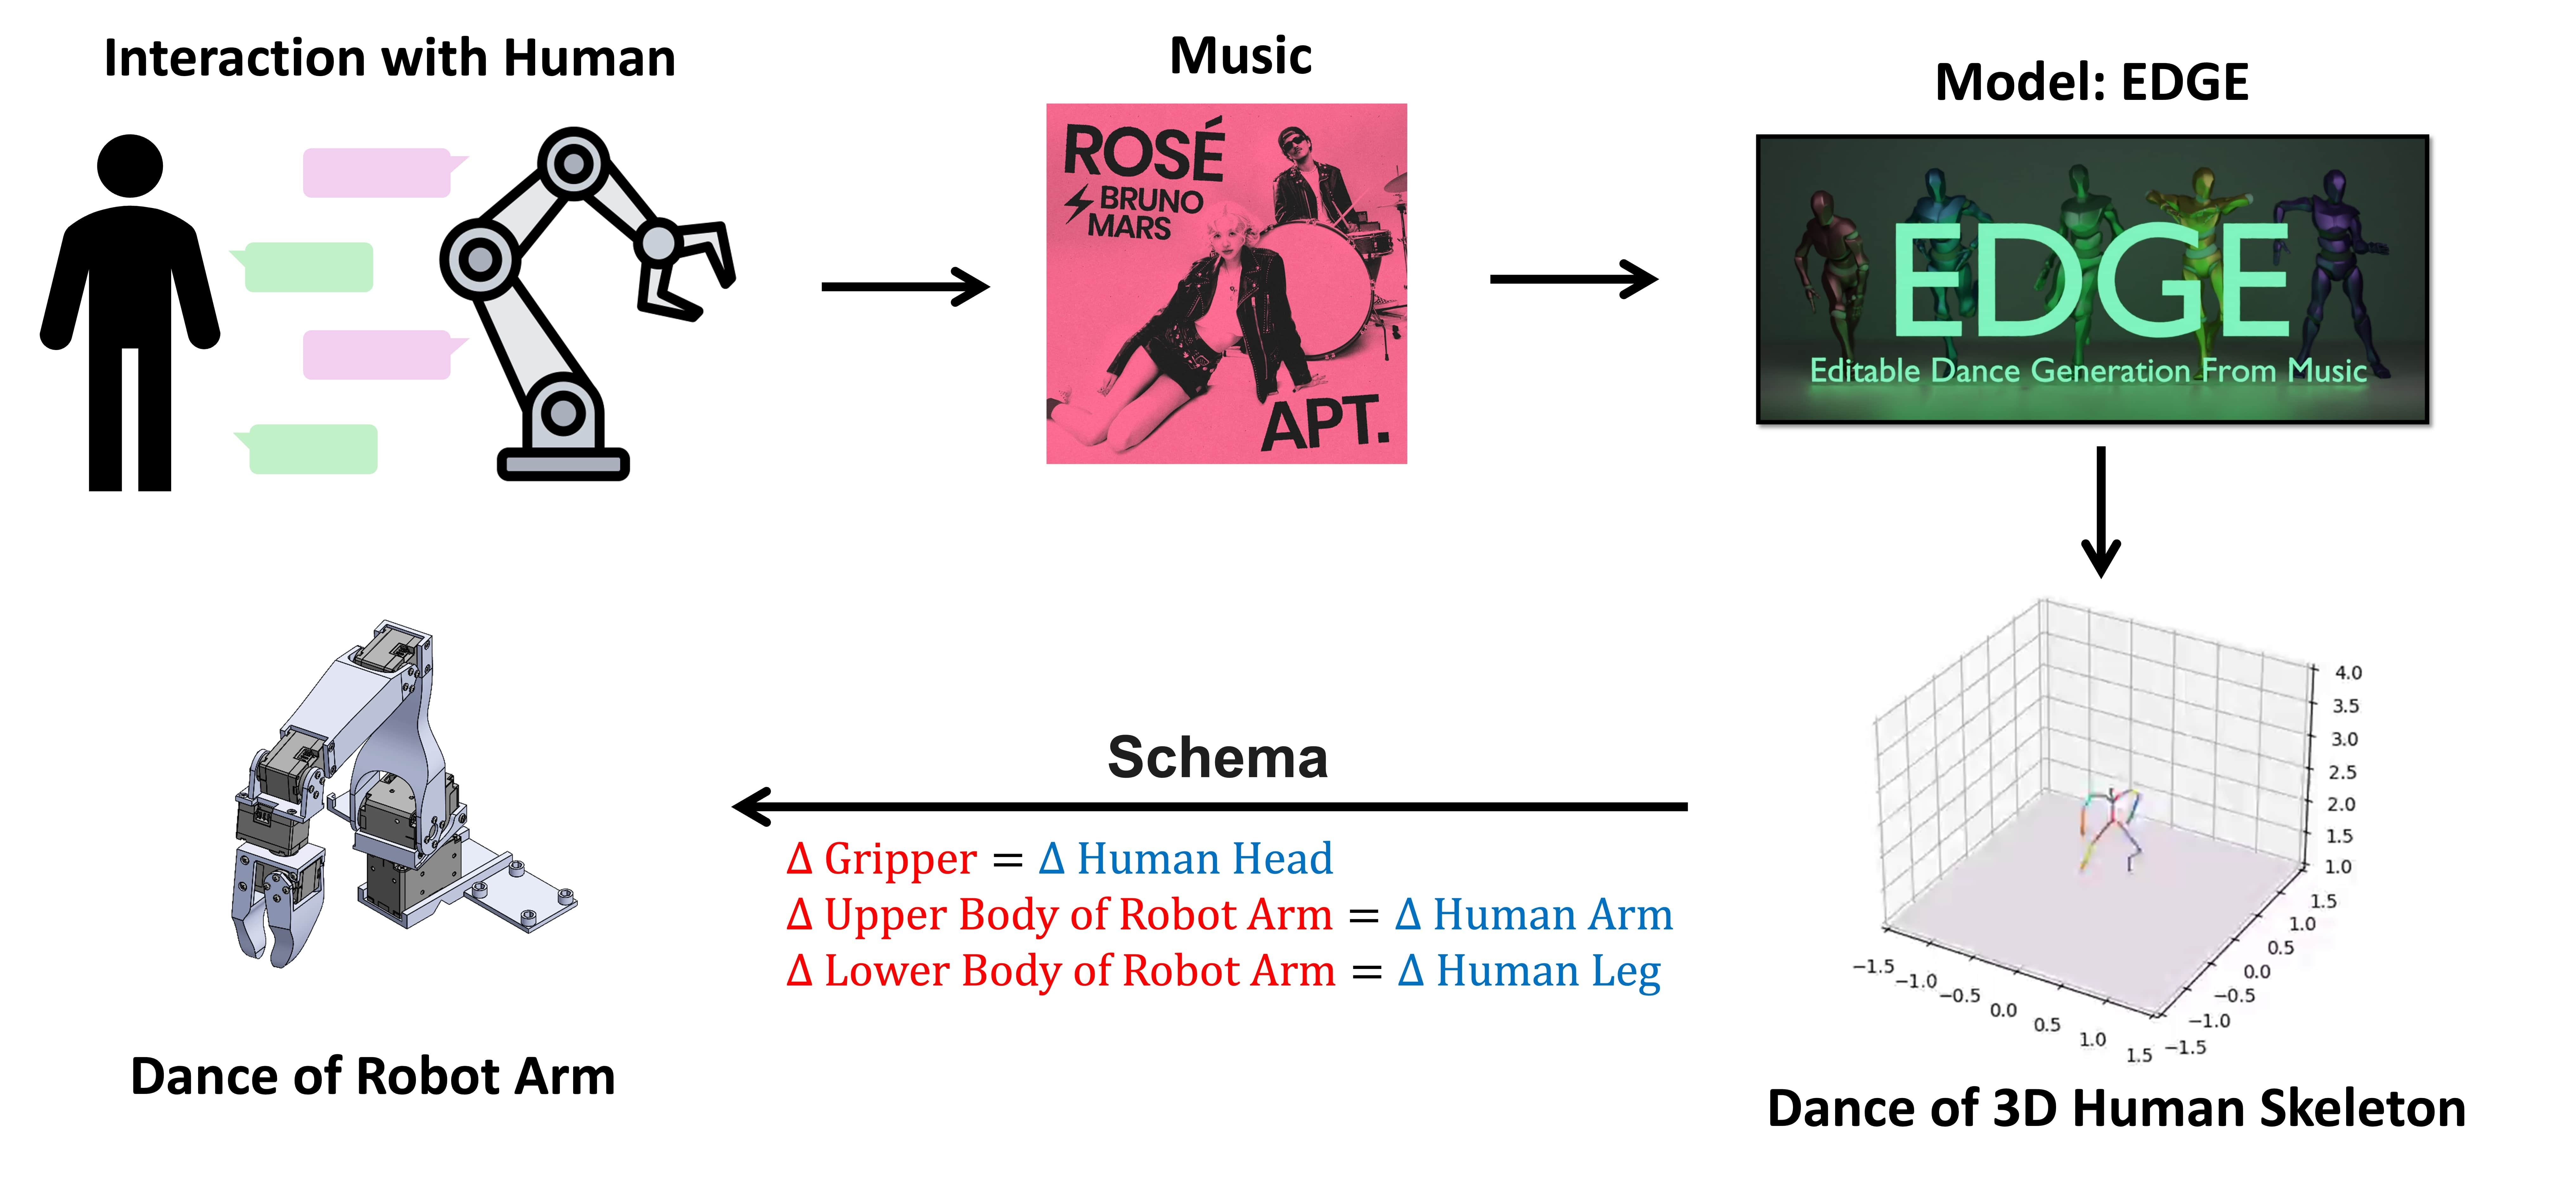
\includegraphics[width=\linewidth]{figures/figure_overview.jpg}
    \caption{Overview of our framework}\label{fig:overview}
\end{figure}

\subsection{Human-Robot Interaction}
For robot dancing, the robot should select proper music. The music is selected by interacting with the human. When human ask something to robot, the robot recognizes human voice and converts it into text using Whisper model \cite{radford2023robust}. Then, GPT model \cite{openai2024gpt4omini} generates the response in a text format based on the text from whisper. Finally, TTS model converts the response text to a audio. Note all conversations between human and robot are in Korean. 

We design 2 types of human-robot interaction scenarios: \texttt{DanceForMe} and \texttt{DanceWithMe}. Fig. \ref{fig:hri_scenario} shows an example of human-robot interaction scenarios. In the \texttt{DanceForMe}, human told robot to dance with calm music. The robot then recommends one of the calm music, “City of Stars”, and the function \texttt{DanceForMe} is executed. \texttt{DanceForMe} function makes the robot dance based on the selected music. In the \texttt{DanceWithMe}, human told that he is happy and he wants to dance. Then, the robot determine the human is in a good mood, and recommend an upbeat music, “APT”, and the function \texttt{DanceWithMe} is executed. \texttt{DanceWithMe} is a function which makes the robot dance when the human is dancing.

\begin{figure}[h]
    \centering
    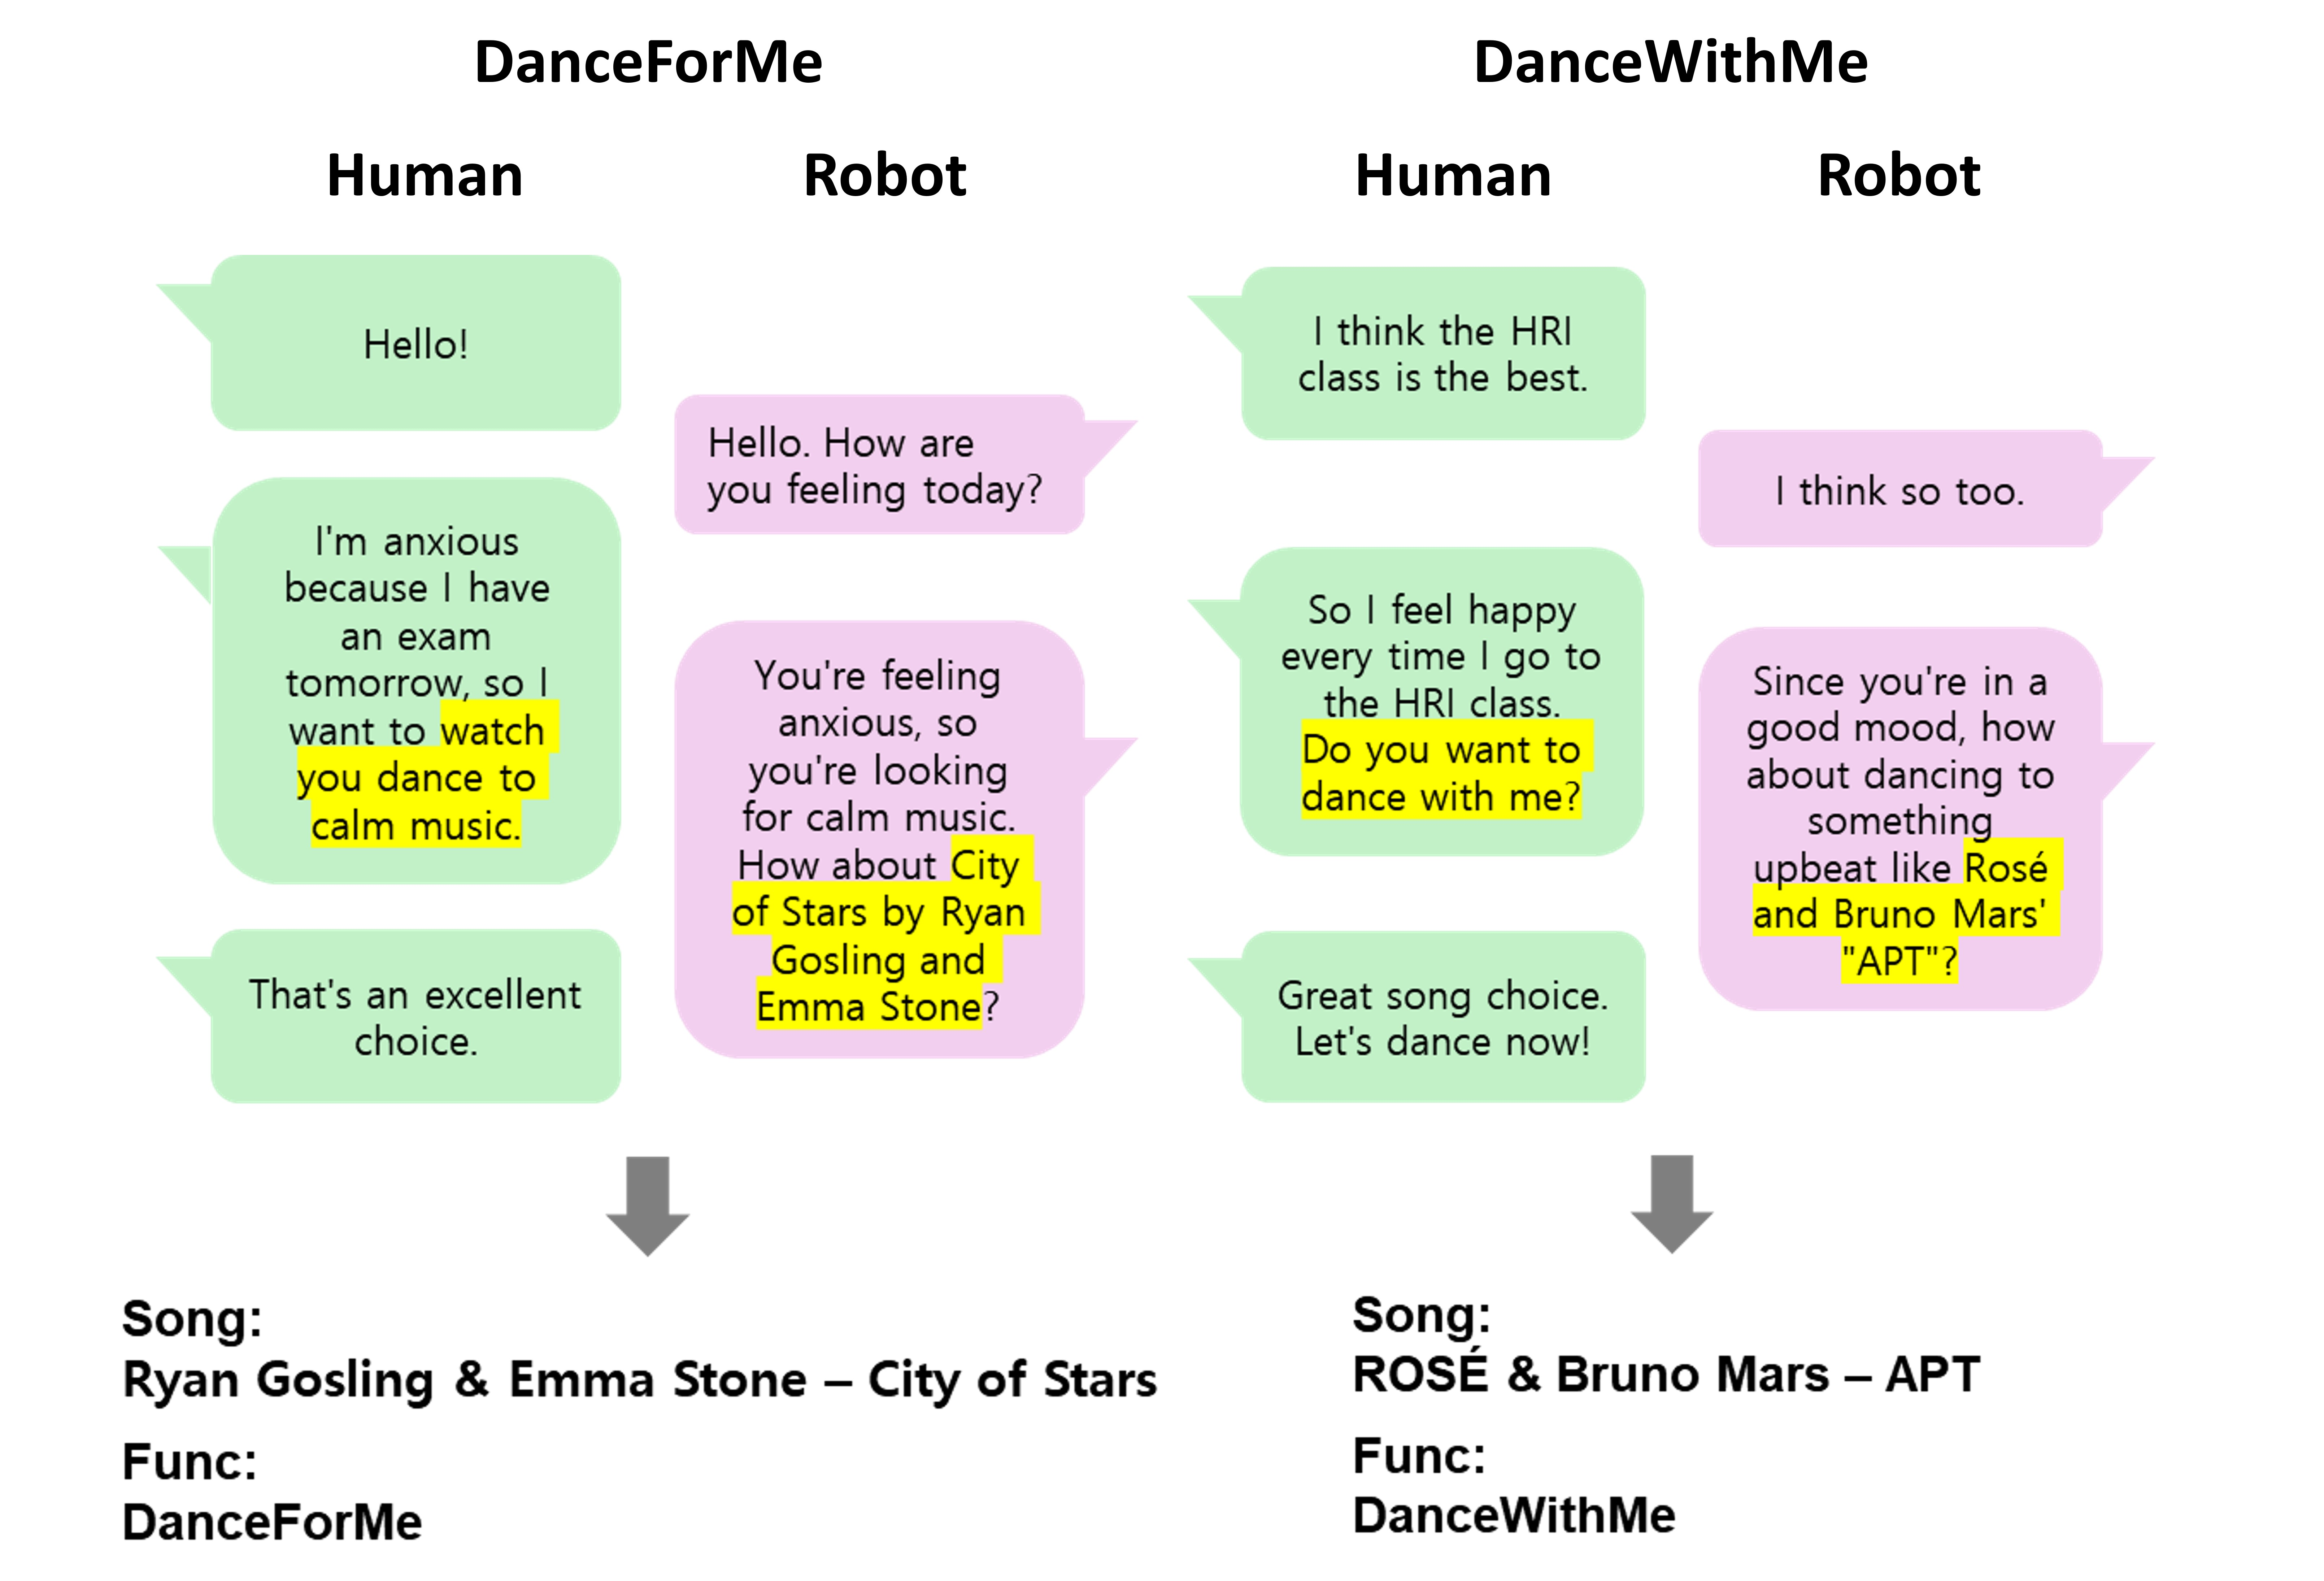
\includegraphics[width=\linewidth]{figures/figure_scenario.jpg}
    \caption{Example of human-robot interaction scenarios. \texttt{DanceForMe} (left). \texttt{DanceWithMe} (right)}\label{fig:hri_scenario}
\end{figure}

In \texttt{DanceWithMe}, the robot dances with the human, which means the robot dances only when the human is dancing. So, the robot should determine whether the human is moving or not. To do so, we use a pose estimation model, YOLOv8 Pose model \cite{Jocher_Ultralytics_YOLO_2023} with a webcam. By calculating the Euclidean distance of joint positions per frame detected by YOLOv8 Pose model, we can effectively detect human movements. However, even in the absence of actual movement, noise can cause the system to detect motion falsely. To solve this, a frame-wise motion detection technique is applied to filter out outliers caused by noise, enabling more accurate movement detection. The frame-wise motion detection technique uses two thresholds to ensure stable and noise-free motion detection. Fig. \ref{fig:human_robot_keypoints} shows how to apply these thresholds in our framework.

\begin{figure}[h]
    \centering
    \begin{subfigure}[b]{\linewidth}
        \centering
        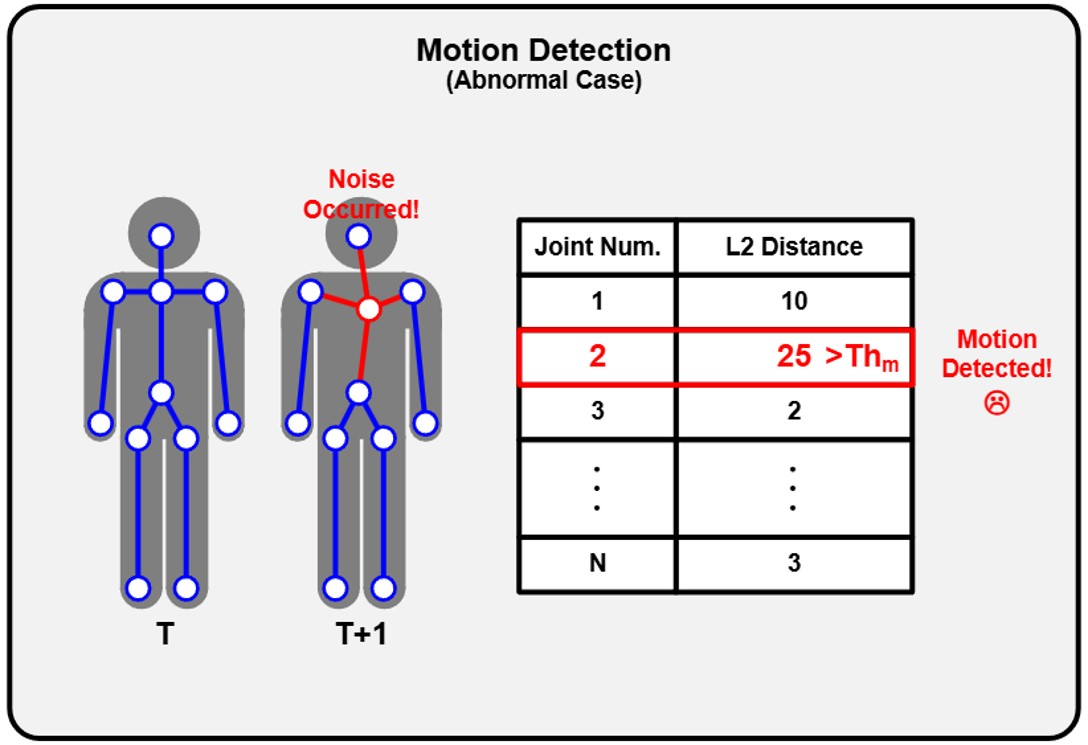
\includegraphics[width=0.7\linewidth]{figures/figure_motion_threshold.jpg}
        \caption{Example of \textit{Motion Threshold}, $Th_{m}$}
    \end{subfigure}
    \hfill
    \begin{subfigure}[b]{\linewidth}
        \centering
        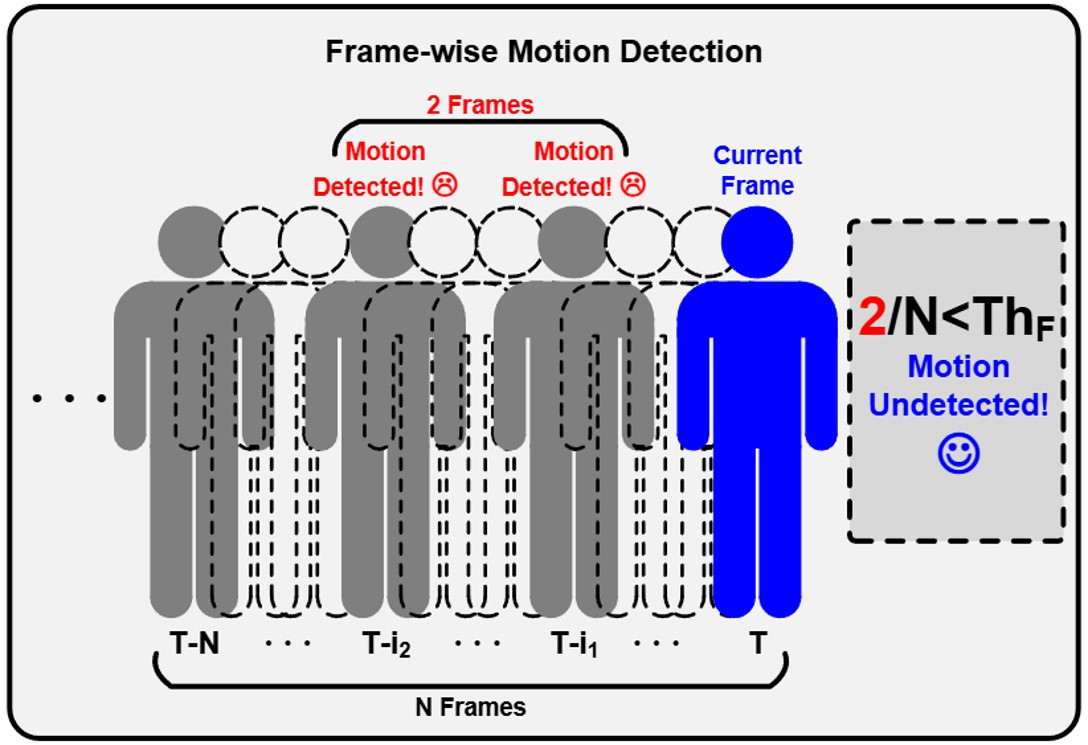
\includegraphics[width=0.7\linewidth]{figures/figure_frame_threshold.jpg}
        \caption{Example of \textit{Frame Threshold}, $Th_{F}$.}
    \end{subfigure}
    \caption{Examples of the frame-wise motion detection technique for accurate human motion detection. (a) \textit{Motion Threshold} determines movement within a single frame based on the Euclidean distance of joint positions. (b) \textit{Frame Threshold} considers a frame as "moving“ only if movement is detected in $k$ frames out for the previous $N$ frames. This approach allows for robust motion detection while filtering out noise.}\label{fig:human_robot_keypoints}
\end{figure}

\subsection{Human Dance from Song}
To generate human-like dance movements from a given song, we employ the EDGE \cite{tseng2023edge} model, which transforms input music into human skeleton motion. We randomly sampled 10 segments of each song at 30-second intervals and used them to generate a human skeleton. The EDGE model outputs human skeletal data in the form of a \texttt{.pkl} file containing 24 keypoints, structured as (frame, keypoints, coordinate). Since the model generates a dance motion with 30Hz, each file has data of dimensions (900, 24, 3).

\subsection{Robot Dance from Human Dance}
The human dance is mapped onto the robot arm's joints through a specific schema, which matches 24 human skeleton keypoints to 6 robot arm keypoints. Fig. \ref{fig:human_robot_keypoints} (a) represents the human skeleton structure and information on joints of robot arm. Detailed matching information between human skeleton and robot joints is in Fig. \ref{fig:human_robot_keypoints} (b).

\begin{figure}[h]
    \centering
    \begin{subfigure}[b]{\linewidth}
        \centering
        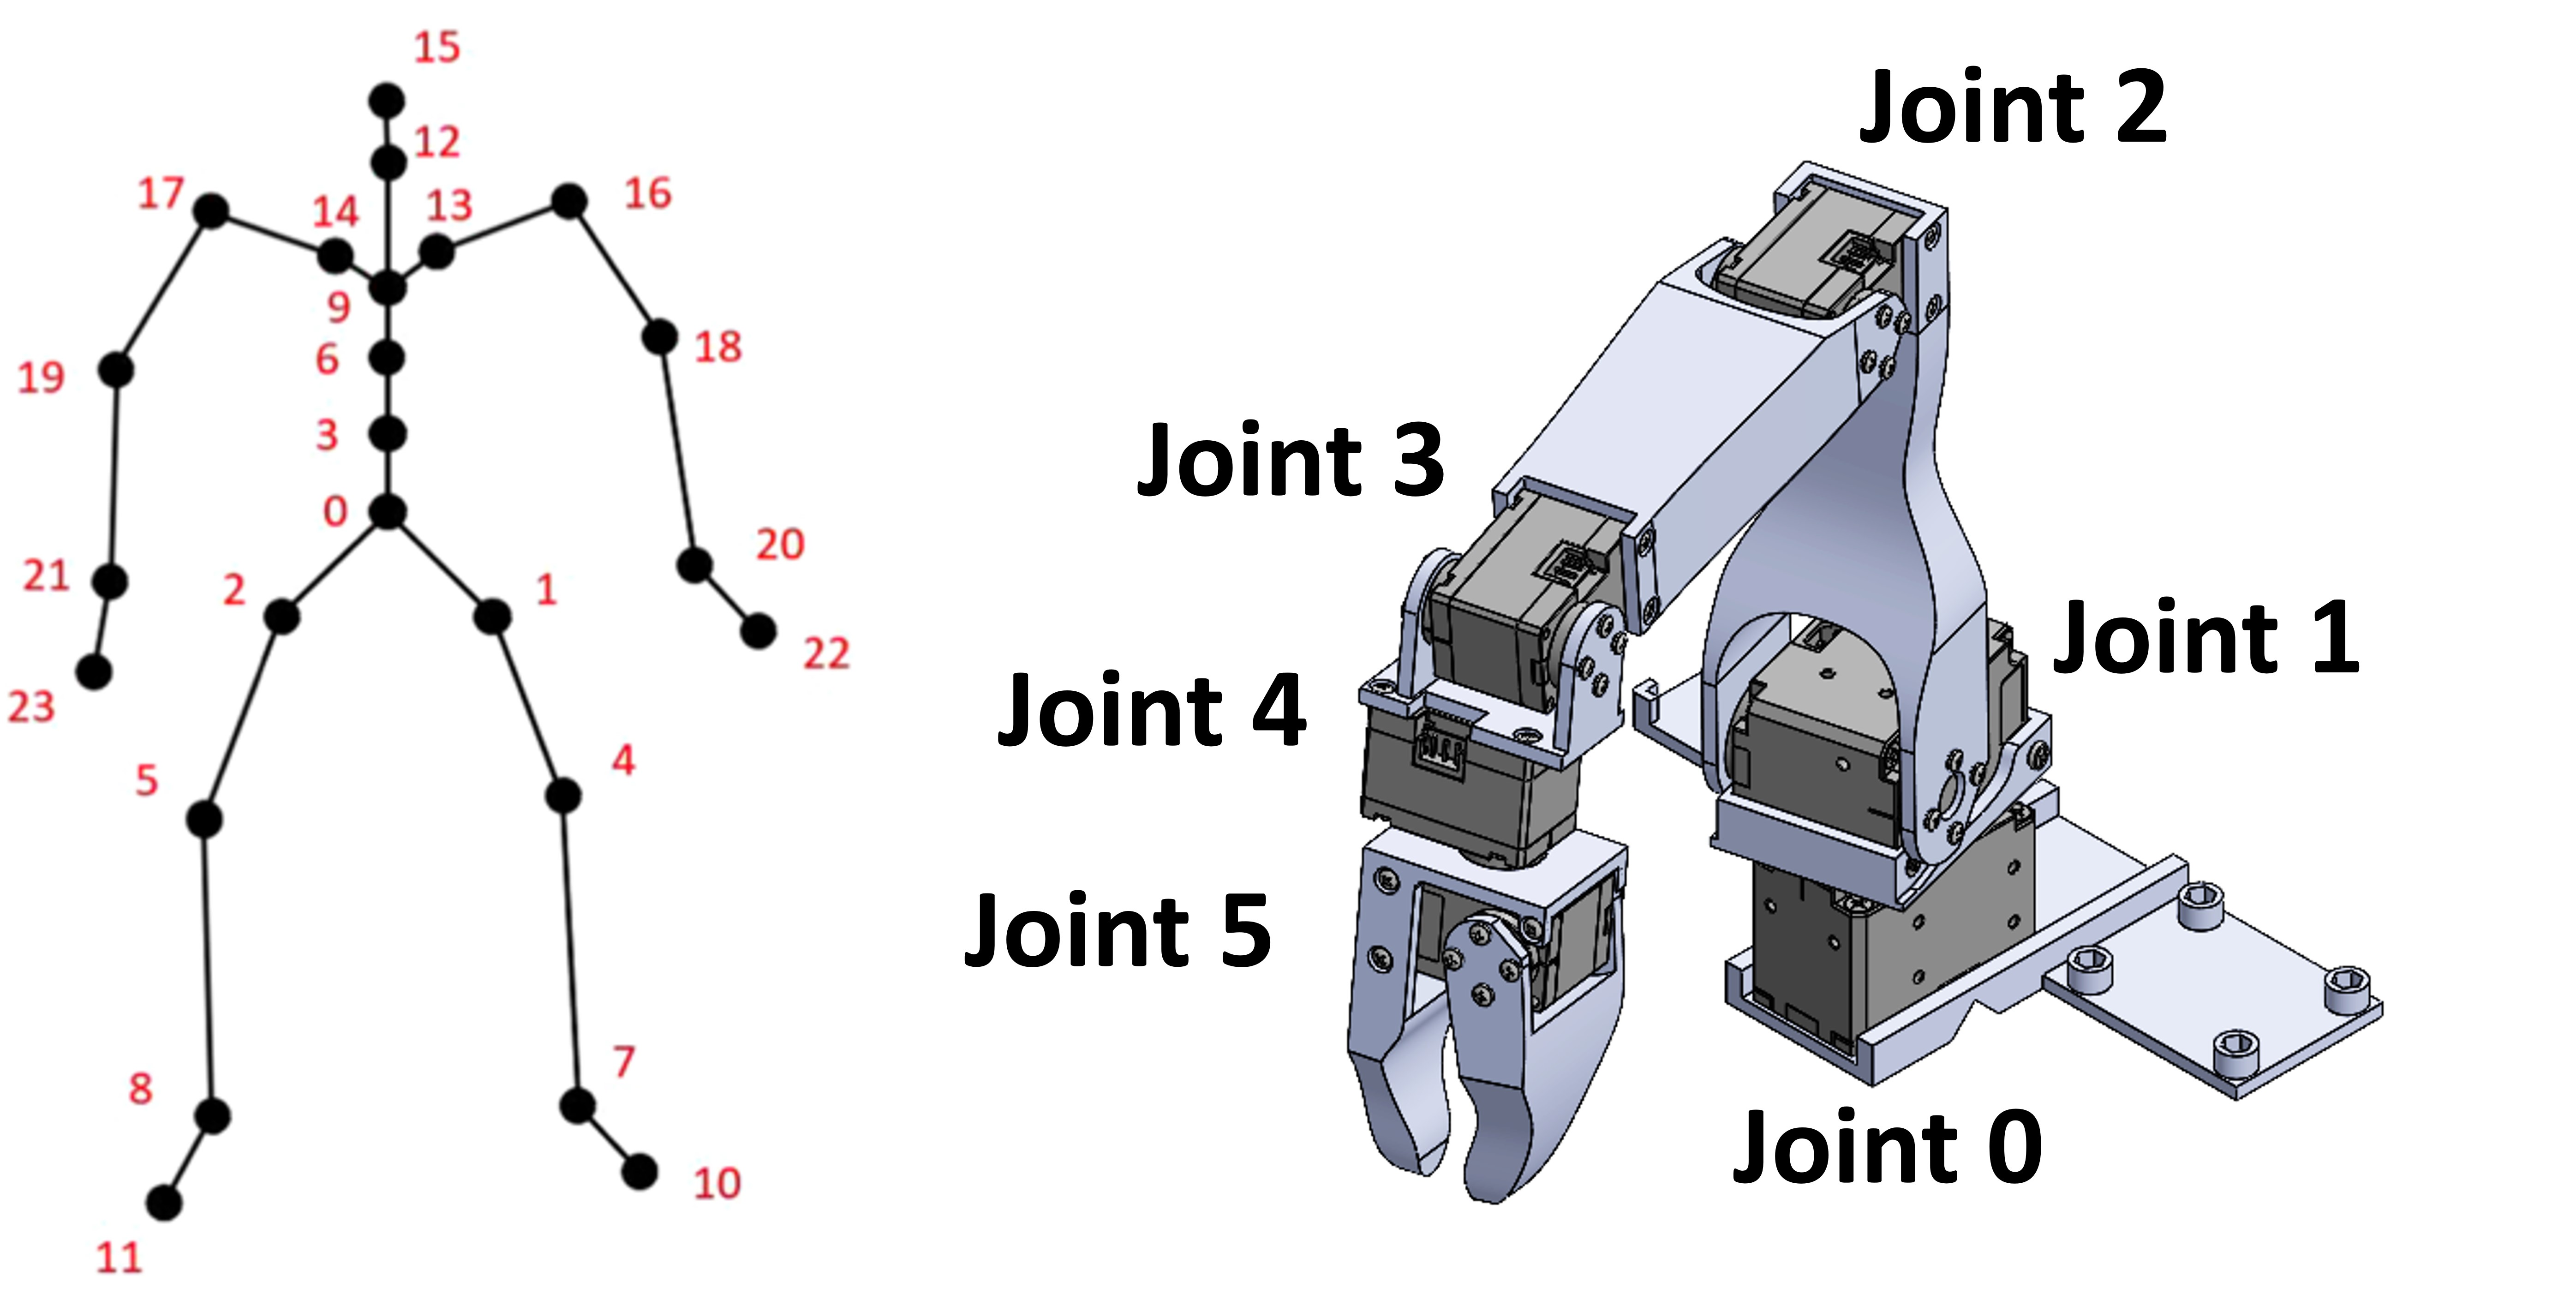
\includegraphics[width=0.7\linewidth]{figures/figure_method_human_robot_matching_1.jpg}
        \caption{}
    \end{subfigure}
    \vfill
    \begin{subfigure}[b]{\linewidth}
        \centering
        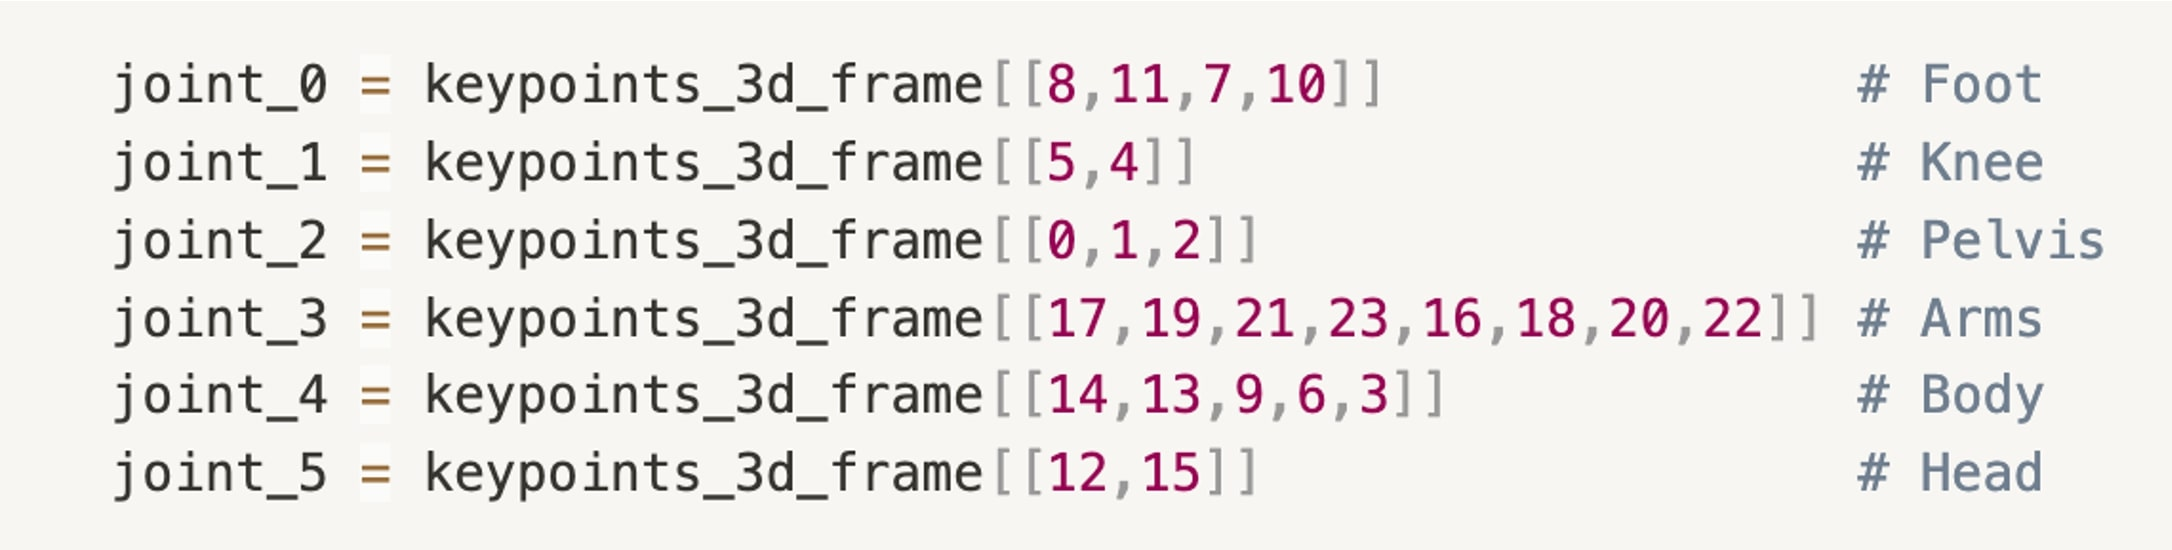
\includegraphics[width=0.9\linewidth]{figures/figure_method_human_robot_matching_2.jpg}
        \caption{}
    \end{subfigure}
    \caption{(a) The structure of 3D human skeleton data generated by EDGE model. There are 24 keypoints per frame in the human skeleton data. (b) Pseudo code for matching keypoints of human to joints of robot.}\label{fig:human_robot_keypoints}
\end{figure}

So, the joint $k$ of robot in the $l^{th}$ frame can be expressed as following: $$W^k_l = [[x_1,y_1,z_1],[x_2,y_2,z_2],...,[x_i,y_i,z_i]],$$ where $i$ represents the number of human motion keypoints consisting joint $k$ of the robot. For reflecting multiple human skeleton motion change to one joint of the robot, we need to calculate the variance for each joint. To do this, we convert the value of each joint in each frame into a single scalar, which represents how much the joint has changed from the initial state, using Frobenius norm. Frobenius norm can be expressed as following:
\begin{align*}
    ||W_{l}|| &= \sqrt{\sum^{m}_{i=1}\sum^{n}_{j=1}|(W_{l})_{i,j}|^{2}}, \\
    ||W_{0}|| &= \sqrt{\sum^{m}_{i=1}\sum^{n}_{j=1}|(W_{0})_{i,j}|^{2}}, \\
    V_{l} &= ||W_{l} - W_{0}||.
\end{align*}
These values $V_{l}$ were normalized to the range of [-1, 1] and mapped to predefined joint angle ranges to avoid motor overload in the joint.

\section{EXPERIMENT}
In this section, we evaluate our framework by comparing the robot dance motion and the human dance motion. It is conducted by measuring synchronization between music's rhythm and dance motion, and user survey.

\subsection{Evaluation Metric}
In the previous work, there are metrics for evaluating generated dance motion such as Generation Diversity (Dist), Frechet Inception Distance (FID), and Physical Foot Contact socre (PFC) \cite{tseng2023edge}, \cite{siyao2022bailando}. However, these are the metric for human motion which is not proper for robot dance motion. So, we analyze our experimental result based on the beat alignment score. It measures how well the generated dance synchronize with the beats of the music by comparing motion features with the rhythm. Beat Alignment score can be expressed as following \cite{siyao2022bailando}:
\begin{align*}
    \text{BeatAlign} = \frac{1}{|B^{m}|}\sum_{t^{m} \in B^{m}}\exp\left(-\frac{\min_{ t^{d}\in B^{d}}||t^{d} - t^{m}||^{2}}{2\sigma^{2}}\right),
\end{align*}
where $B^{d}$, $B^{b}$, $\sigma$ represent the time of beats in dance, the time of beats in music, and normalized parameter, respectively.


\subsection{User Survey}
As well as measuring metric, we conduct user survey about our dancing robot, to evaluate how much the generated dance looks like a dance from the perspective of human. There are 2 types of sections in the survey. Fig. \ref{fig:survey_form} shows the example of our survey. In the first section, we show the video that the robot dances mimicking human dance. We receive responses to questions about asking similarity between robot and human dance. In the second section, we show the video that the robot dances with the background music. One of the robots is the output of our framework which generated robot dance based on the music, and another one is a fake data which is not generated based on the music. We receive responses to questions about asking each robot fits to music well.

\begin{figure}[h]
    \centering
    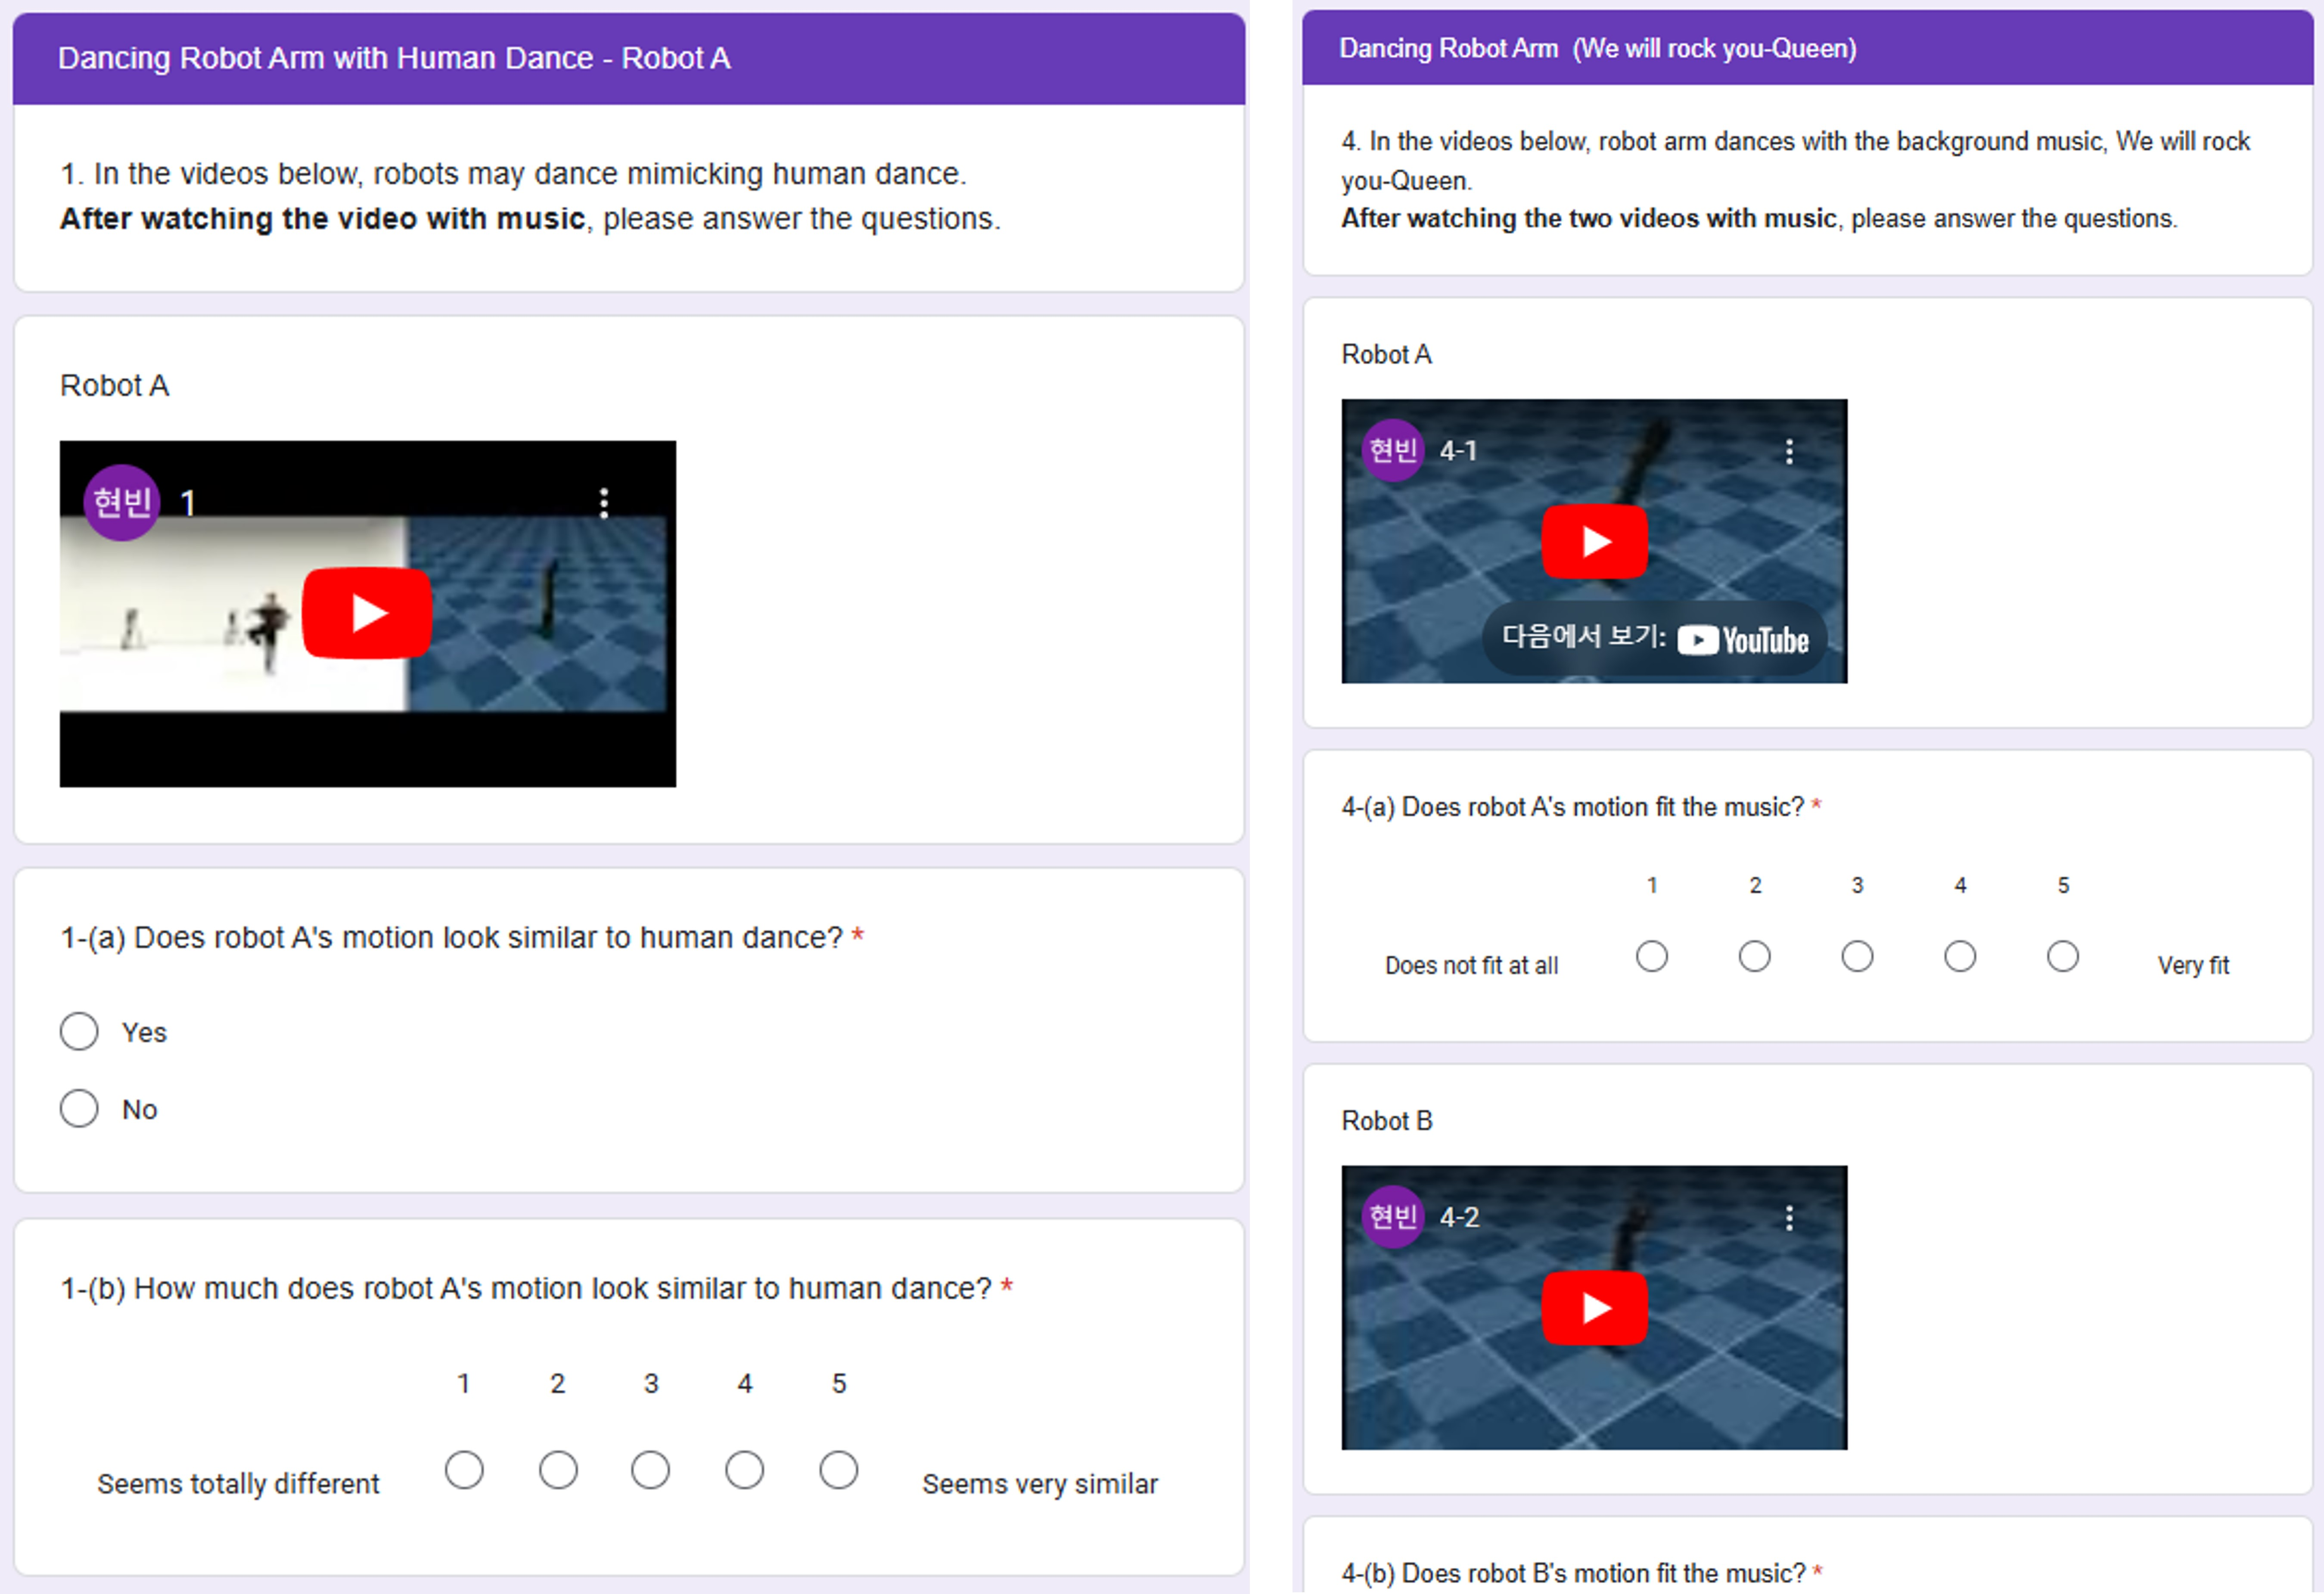
\includegraphics[width=\linewidth]{figures/figure_survey.jpg}
    \caption{Example of survey form. There are 41 responses in the survey.}\label{fig:survey_form}
\end{figure}


\subsection{Results and Analysis}

\begin{figure}[!h]
    \centering
    \begin{subfigure}[b]{\linewidth}
        \centering
        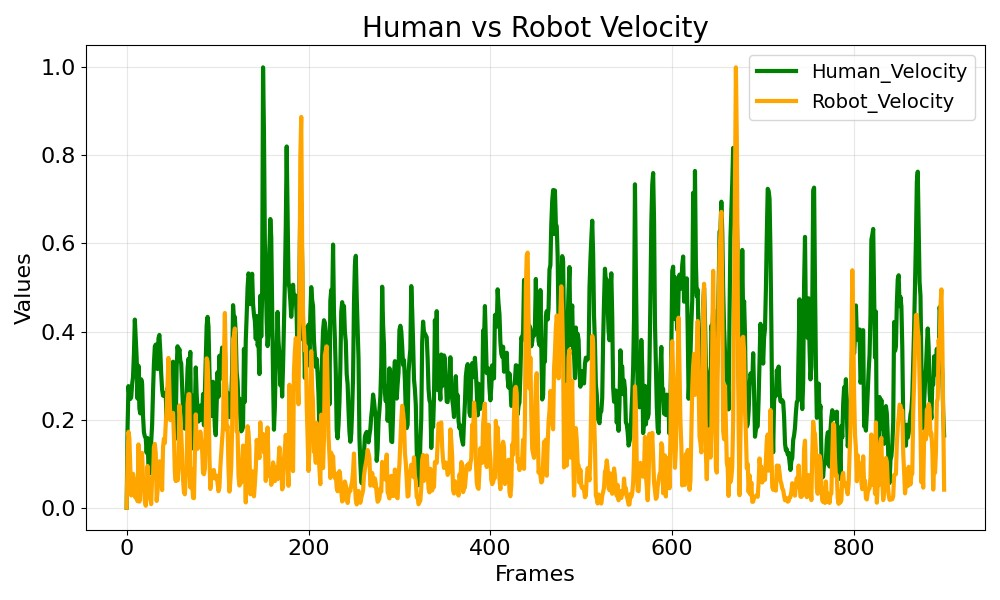
\includegraphics[width=0.9\linewidth]{figures/figure__last_christmas_velocity.jpg}
        \caption{tmp}
    \end{subfigure}
    \vfill
    \begin{subfigure}[b]{\linewidth}
        \centering
        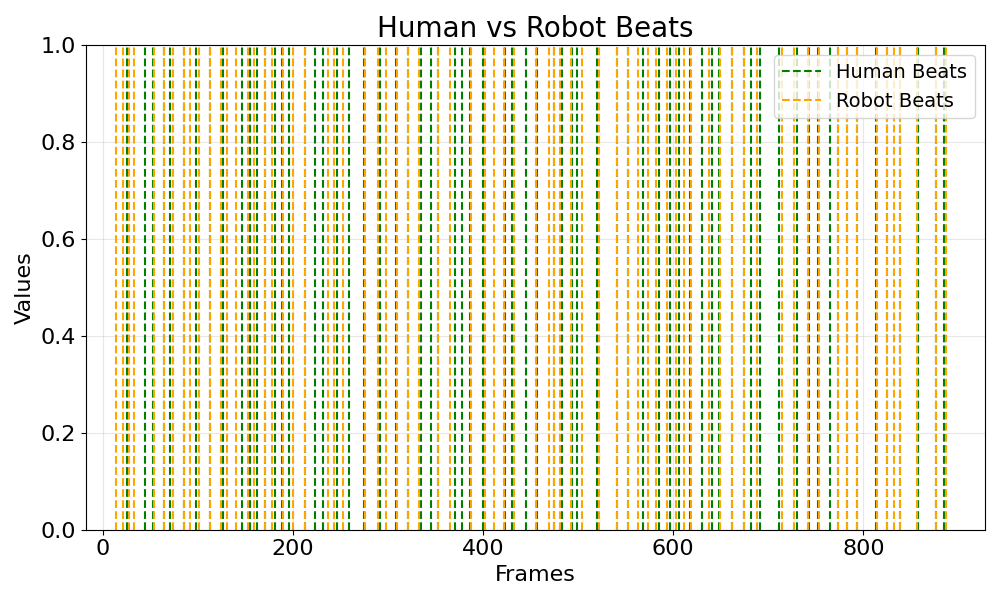
\includegraphics[width=0.9\linewidth]{figures/figure__last_christmas_beats.png}
        \caption{tmp}
    \end{subfigure}
    \caption{tmp}\label{fig:result_last_christmas}
\end{figure}

\begin{table}[h!]
\centering
\resizebox{\columnwidth}{!}{
\begin{tabular}{ccc}
\Xhline{2\arrayrulewidth}
\textbf{Music} & \textbf{Human Dance (EDGE \cite{tseng2023edge})} & \textbf{Robot Dance (Ours)} \\ \hline \hline 
Another Day Of Sun & 0.4448 & 0.4349 \\ \hline
APT & 0.5662 & 0.5373 \\ \hline
Bang Bang Bang & 0.5959 & 0.5638 \\ \hline
Last Christmas & 0.4493 & 0.4409 \\ \hline
City Of Star & 0.3973 & 0.4057 \\ \hline
Million Dollar Baby & 0.3836 & 0.3932 \\ \hline
Still Life & 0.5005 & 0.5136 \\ \hline
We Will Rock You & 0.3227 & 0.2793 \\ 
\Xhline{2\arrayrulewidth}
\end{tabular}}
\caption{Beat Alignment Score for Human and Robot Dance}
\label{table:beat_alignment}
\end{table}


\begin{table}[h!]
\centering
\resizebox{\columnwidth}{!}{
\begin{tabular}{ccccc}
\Xhline{2\arrayrulewidth}
\textbf{Sample ID} & \textbf{Beats} & \textbf{Velocity} & \textbf{Max Velocity} & \textbf{Min Velocity} \\ \hline \hline
Sample 1 & 1.0 & 0.1035 & 0.4584 & 0 \\ \hline
Sample 2 & 1.0 & 0.2147 & 0.9464 & 0 \\ \hline
Sample 3 & 1.0 & 0.1224 & 0.7584 & 0 \\ \hline
Sample 4 & 1.0 & 0.2112 & 0.7598 & 0 \\ \hline
Sample 5 & 1.0 & 0.1779 & 0.8976 & 0 \\ \hline
Sample 6 & 1.0 & 0.2243 & 0.8784 & 0 \\ \hline
Sample 7 & 1.0 & 0.0984 & 0.6303 & 0 \\ \hline
Sample 8 & 1.0 & 0.2353 & 0.8258 & 0 \\ \hline
Sample 9 & 1.0 & 0.1981 & 0.8321 & 0 \\ \hline
Sample 10 & 1.0 & 0.2048 & 0.8325 & 0 \\ \Xhline{2\arrayrulewidth}
\end{tabular}}
\caption{Comparison of Human and Robot Dance by Velocity and Beats}
\label{table:exp1_beat_alignmnet_score}
\end{table}




tmp



\section{CONCLUSION}
In this project, we present the framework for the human-robot interaction with the dancing robot arm. Our framework shows that the robot dances in sync with any kind of music, and interacts with humans in two ways. One is that the robot recommends music and dances for human by communicating with human. The other is that the robot detects human movements and dances collaboratively with human. Experiment results show that the robot's dance aligns well with the music's beat, and the robot's dance fits the music but does not closely mimic human movements. For future work, we aim to improve human-to-robot motion mapping and explore methods to better reflect human-like movements.

\bibliographystyle{IEEEtran}
\bibliography{main.bib}

\end{document}
